\subsubsection{Attitude Controller Simulation}

\begin{figure}[H]
	\centering
	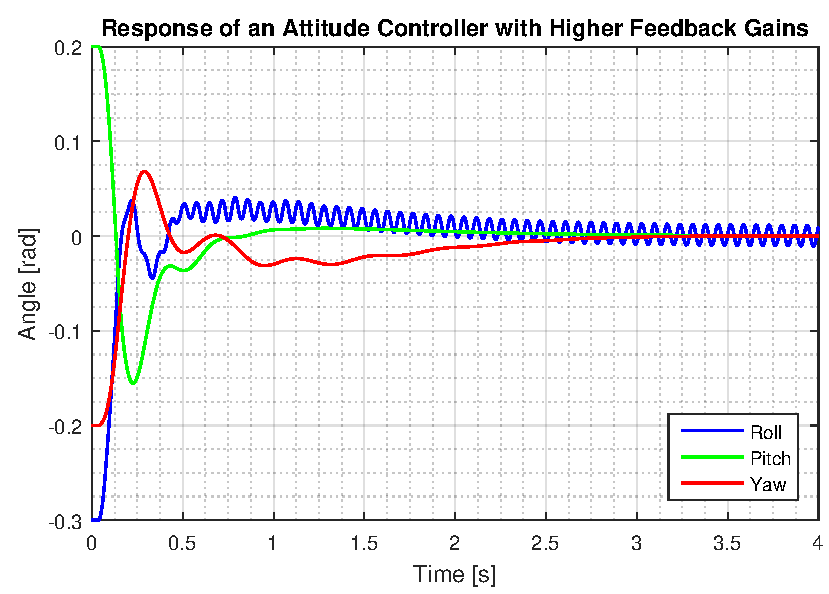
\includegraphics[scale=1]{figures/ssEqBad.pdf}
	\caption{.}
	\label{fig:TranslationalControlDiagram}
\end{figure}

\begin{flalign}
    \vec{Q}_{9 \times 9} =	 
    \begin{bmatrix}
        \ 1/0.1^2 & 0 & 0 & 0 & 0 & 0 & 0 & 0 & 0     	\ \ \ \\ 
        \ 0 & 1/0.1^2 & 0 & 0 & 0 & 0 & 0 & 0 & 0     	\ \ \ \\ 
        \ 0 & 0 & 1/0.1^2 & 0 & 0 & 0 & 0 & 0 & 0     	\ \ \ \\
        \ 0 & 0 & 0 & 1/0.4^2 & 0 & 0 & 0 & 0 & 0 		\ \ \ \\
        \ 0 & 0 & 0 & 0 & 1/0.5^2 & 0 & 0 & 0 & 0		\ \ \ \\
        \ 0 & 0 & 0 & 0 & 0 & 1/0.3^2 & 0 & 0 & 0 		\ \ \ \\
        \ 0 & 0 & 0 & 0 & 0 & 0 & 1/0.08^2 & 0 & 0 		\ \ \ \\
        \ 0 & 0 & 0 & 0 & 0 & 0 & 0 & 1/0.08^2 & 0 		\ \ \ \\
        \ 0 & 0 & 0 & 0 & 0 & 0 & 0 & 0 & 1/0.05^2	 	\ \ \ \\
    \end{bmatrix} \nonumber
\end{flalign}

\begin{flalign}
    \vec{R}_{3 \times 6} =	 
    \begin{bmatrix}
        \ 1/65^2 & 0 & 0 & 0      \ \ \ \\ 
        \ 0 & 1/65^2 & 0 & 0     \ \ \ \\ 
        \ 0 & 0 & 1/65^2 & 0      \ \ \ \\	
        \ 0 & 0 & 0 & 1/65^2      \ \ \ \\	
    \end{bmatrix} \nonumber
\end{flalign}

\begin{figure}[H]
	\centering
	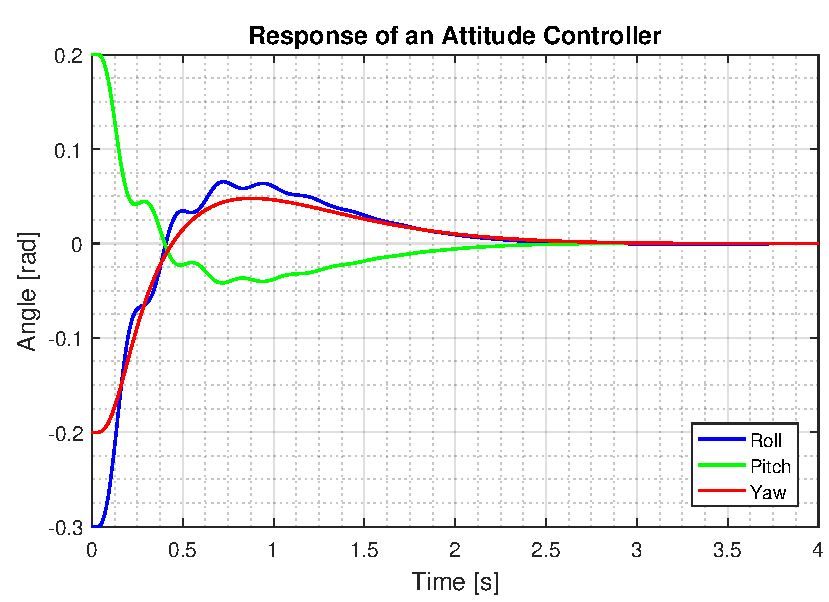
\includegraphics[scale=0.8]{figures/ssFinalEq.pdf}
	\caption{.}
	\label{fig:TranslationalControlDiagram}
\end{figure}



\begin{figure}[H]
	\centering
	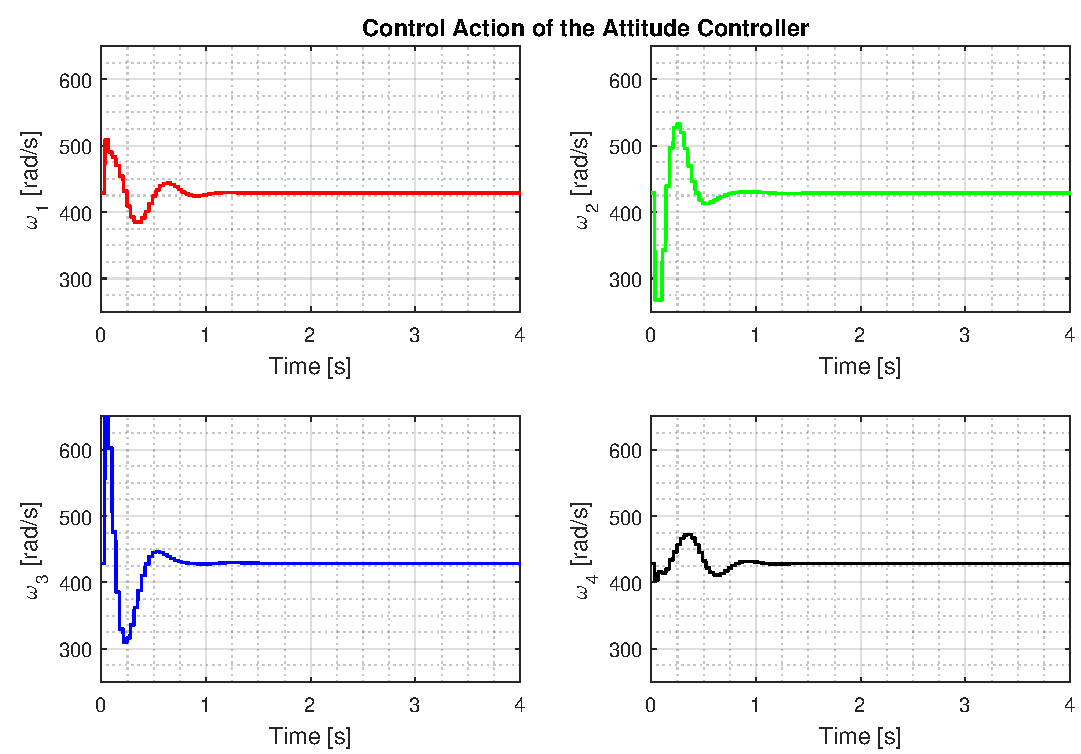
\includegraphics[scale=0.8]{figures/ssFinalEqAction.pdf}
	\caption{.}
	\label{fig:TranslationalControlDiagram}
\end{figure}

\begin{figure}[H]
	\centering
	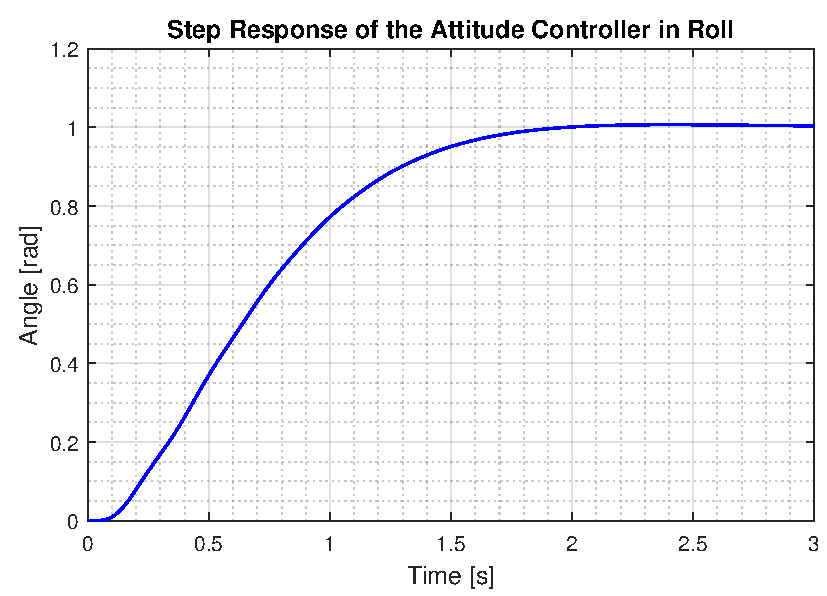
\includegraphics[scale=0.8]{figures/ssFinalStep.pdf}
	\caption{.}
	\label{fig:TranslationalControlDiagram}
\end{figure}

\begin{figure}[H]
	\centering
	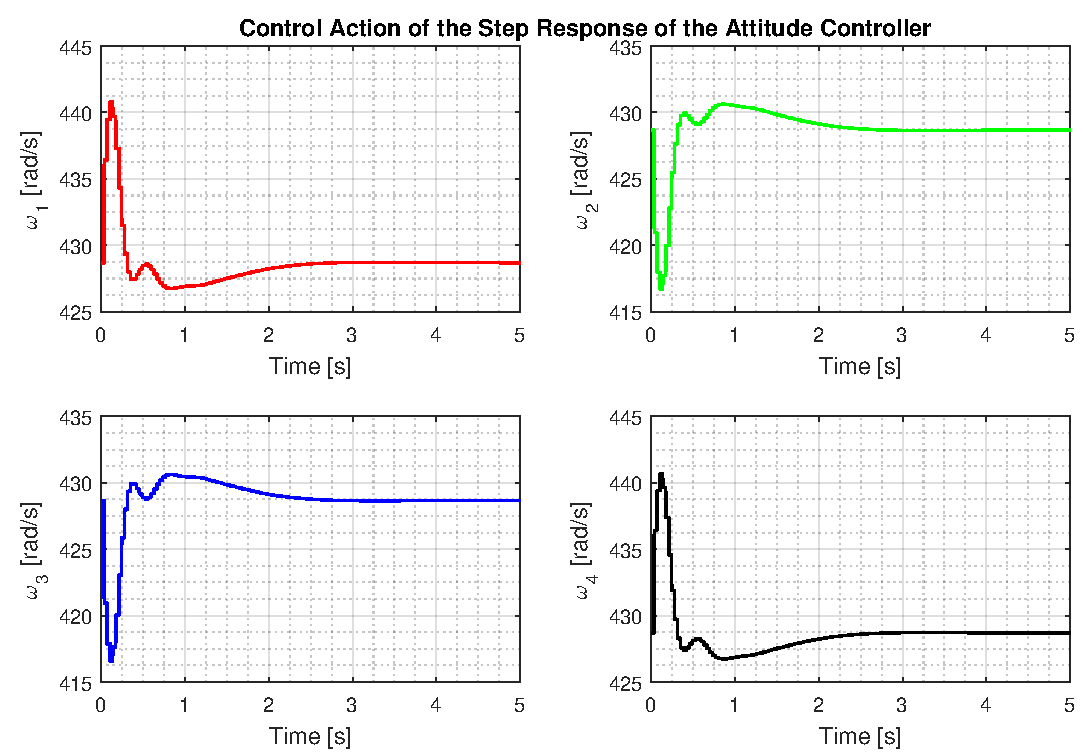
\includegraphics[scale=0.8]{figures/ssFinalStepAction.pdf}
	\caption{.}
	\label{fig:TranslationalControlDiagram}
\end{figure}